% !TeX root = main.tex

% ============================================================
% thesis-sync entry: 2026-07-06_lizard-robot-architecture
% Type: design decision + numeric data
% Insertable section block (no preamble). Requires: graphicx, multirow (for tables).
% Figure \includegraphics lines are COMMENTED so the file compiles standalone;
% uncomment and fix the path (figures/<filename>) once images are in the repo.
% ============================================================

\section{LIZARD-INSPIRED SOFT ROBOT: SYSTEM ARCHITECTURE}
\label{sec:lizard-architecture}

\subsection{Design Concept}

The proposed robot is a lizard-inspired, tethered pneumatic soft robot
designed for surface locomotion and for transitions between intersecting
planes. The architecture integrates two actuation subsystems that were
previously developed and characterized in isolation: (i) a coupled
body--tail unit composed of two geometrically identical three-chambered
omnidirectional bending segments, derived from the miniaturization of the
fiber-reinforced actuator presented in Section~\ref{sec:inchworm-actuator}, and
(ii) four single-chambered fiber-reinforced bending legs, each terminating
in an actively evacuated suction-cup foot. Whereas gecko-inspired soft
climbers such as \cite{Schiller2019GeckoInspired} employ a single planar
bending torso, the present design pneumatically couples two
omnidirectional segments through a central connector, so that a single
pressure input can generate either an S-shaped planar deformation of the
body--tail axis (relevant for fundamental forward gait and steering gait) or a U-shaped out-of-plane deformation
(relevant for wall-transition gait), depending on which chamber pair is addressed.
The working hypothesis motivating this architecture is that the coupled
body--tail unit contributes actively to locomotion and posture control,
rather than just serving as a passive structural link.

\subsection{Overall Layout and Global Specifications}

The robot consists of a body segment and a tail segment joined by a rigid
central connector, four leg actuators attached in a sprawled
lizard-like configuration (two anterior, two posterior), four suction-cup
feet, and the pneumatic supply tubing. All soft components are silicone
elastomers: the actuator bodies are cast in translucent EcoFlex 00-30,
whereas the end caps, foot interfaces, and suction cups are cast in
reddish Elastosil M4601 (see Section~\ref{sec:lizard-materials}).
The global specifications, measured with all actuators in the relaxed
state ($P = 0$), are summarized in Table~\ref{tab:lizard-global-specs}.

\begin{table}[tb]
  \caption{Global specifications of the lizard-inspired soft robot,
  measured in the relaxed state ($P=0$).}
  \label{tab:lizard-global-specs}
  \centering
  \begin{tabular}{|l|c|c|}
    \hline
    Parameter & Value & Unit \\ \hline
    Total mass (without tip loads) & 5.8 & g \\ \hline
    Body-tip to tail-tip length & 85 & mm \\ \hline
    Leg-tip to leg-tip span (incl. suction cups) & 89 & mm \\ \hline
    Total height & 8 & mm \\ \hline
    Number of legs & 4 & -- \\ \hline
    Number of suction-cup feet & 4 & -- \\ \hline
    Body/tail segment: overall actuator length & 33 & mm \\ \hline
    Body/tail segment: silicone tube length & 26 & mm \\ \hline
    Body/tail segment: outer diameter & 6 & mm \\ \hline
    Leg actuator: overall length & 30 & mm \\ \hline
    Leg actuator: silicone tube length & 24 & mm \\ \hline
    Suction cup: outer diameter & 10 & mm \\ \hline
    Suction cup: internal vacuum height & 3 & mm \\ \hline
  \end{tabular}
\end{table}

The low total mass (5.8~g) is a direct consequence of the threefold
miniaturization of the three-chambered actuator relative to
the inchworm actuator of Section~\ref{sec:inchworm-actuator} (see
Section~\ref{sec:lizard-characterization}), and is a relevant figure of
merit for climbing: the adhesion demand on each suction cup scales with
the supported weight, and gecko-inspired soft climbers of comparable
architecture have been reported at total masses of 150--200~g
\cite{Schiller2019GeckoInspired}, more than an order of magnitude heavier.

\subsection{Operating Regime}

All actuators are driven pneumatically at low gauge pressures. In the
robot experiments, the coupled body--tail unit is operated at
approximately 11~kPa, at which each segment reaches a bending angle of
approximately 75$^{\circ}$; the leg actuators reach approximately
90$^{\circ}$ at 13~kPa. These operating points are deliberately far below
the characterization limit of the isolated three-chambered segment, which
reaches a bending angle of approximately 180$^{\circ}$ at 15~kPa when a
single chamber is pressurized (Section~\ref{sec:lizard-characterization});
the margin limits the risk of fiber slippage and seam rupture during
repeated gait cycles. The suction-cup feet are actively evacuated by the
same multichannel pneumatic supply used for the positive-pressure
channels, with vacuum applied in place of positive pressure.

% --- Figures (paths to be fixed by the author; commented for compilation) ---
\begin{figure}[tb]
  \centering
  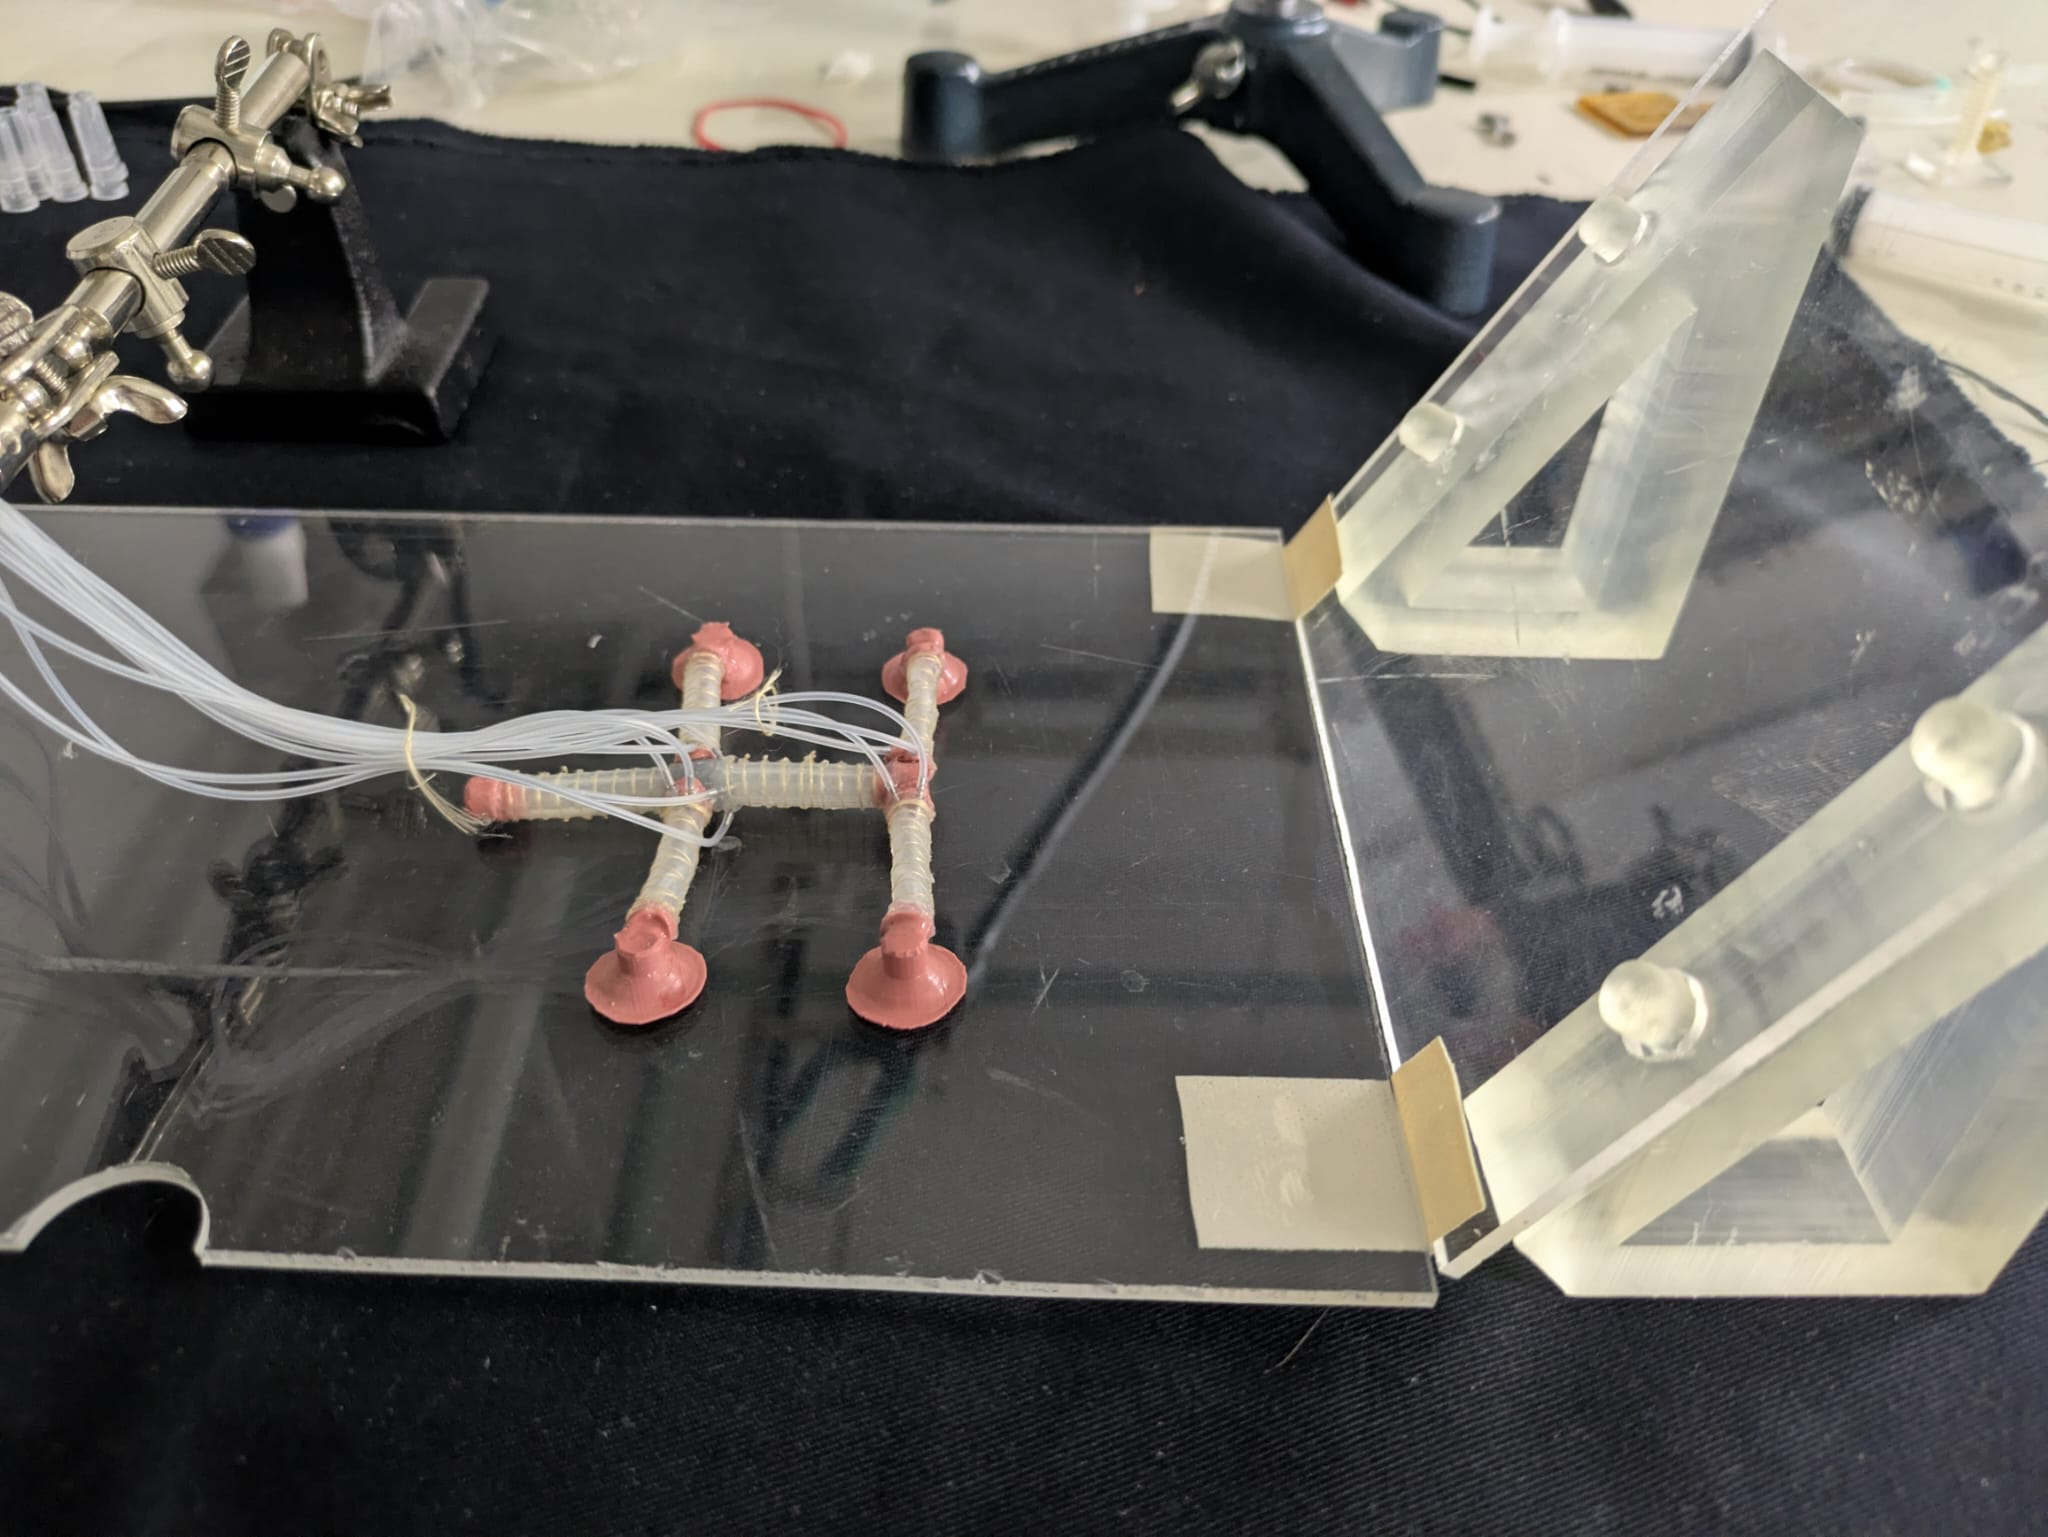
\includegraphics[width=0.95\columnwidth]{figures/lizardExperimentSetup.jpeg}
  \caption{The assembled lizard-inspired soft robot resting on the
  transparent acrylic locomotion plane, with the inclined transition
  substrate visible in the background. The four legs terminate in
  Elastosil M4601 suction-cup feet; the coupled body--tail unit spans the
  central connector.}
  \label{fig:lizard-overview}
\end{figure}

\begin{figure}[tb]
  \centering
  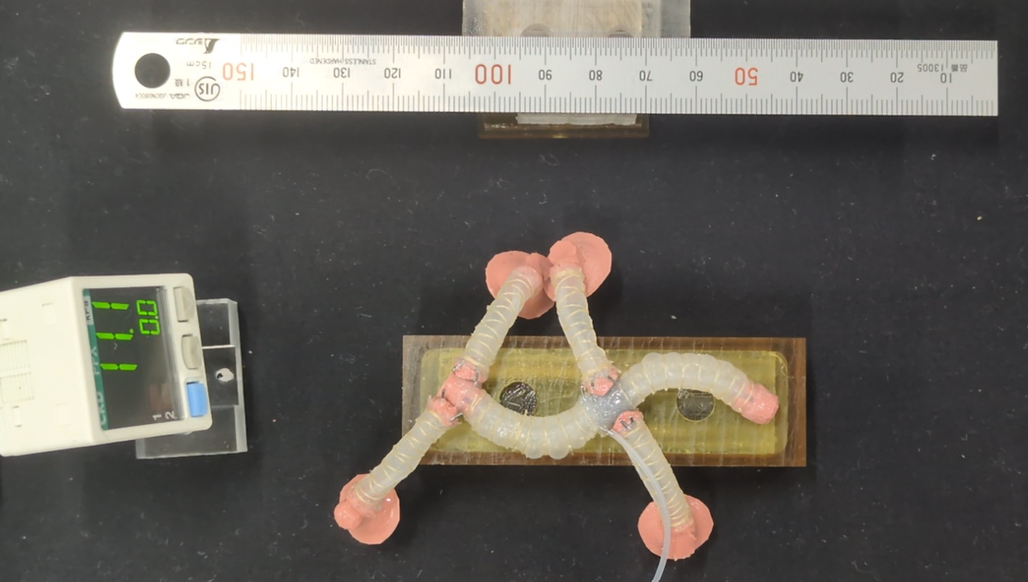
\includegraphics[width=0.95\columnwidth]{figures/Sbodydown11.1.png}
  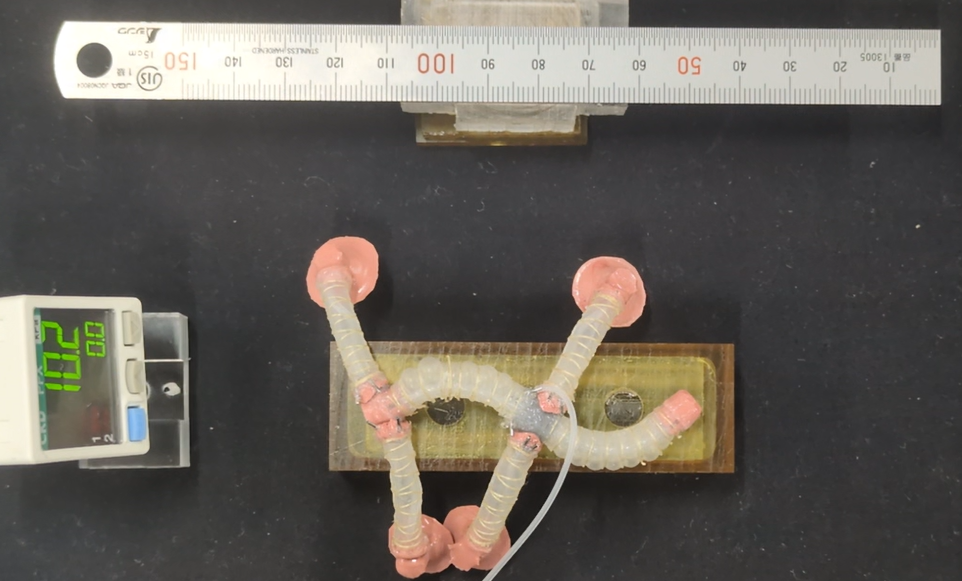
\includegraphics[width=0.95\columnwidth]{figures/Sbodyup10.2.png}
  \caption{Top view of the robot performing horizontal S-shaped bending of
  the body--tail axis at approximately 11.0~kPa (top) and 10.2~kPa
  (bottom), with opposite curvature assignments of the two segments. The
  digital pressure display and a steel rule (150~mm) are included in the
  frame for pressure--deformation correlation and scale.}
  \label{fig:lizard-s-topviews}
\end{figure}
